% 来源: 19c9fbc3-e182-829e-8000-00002574d509_3.2_交换.pdf
% 提取时间: 2026-02-28T22:51:48+08:00

3.2 交换
电路交换
电路交换（Circuit Switching）是一种通信网络技术，其核心思想是在通信双方之间建立一条专用
的物理通信路径（电路），该路径在通信过程中始终保持连接状态，直到通信结束后才会释放。这
种技术类似于传统电话系统的工作方式，例如拨打固定电话时，电话交换机会在通话双方之间建立
一条独占的物理线路。
工作原理
电路交换的工作过程主要包括以下三个阶段：
1.   建立连接阶段
     ○ 发送方向网络发出连接请求，请求中包含接收方的地址信息。
     ○ 网络通过中间节点（如交换机）逐步建立从发送方到接收方的端到端物理连接，这条线路

       在通信期间由双方独占。
     ○ 示例：传统电话网络中，用户拨号后，交换机通过布线建立通话双方的物理线路。

2.   数据传输阶段
     ○ 连接建立完成后，数据通过这条专用线路进行传输，传输过程中无需进行路由选择，数据
       按顺序直达对方。
     ○ 特点：传输延迟低、数据顺序稳定，但线路利用率可能较低（即使无数据传输，线路也被

       占用）。
3.   连接释放阶段
     ○   通信结束后，双方中的任意一方发起断开请求，网络拆除已建立的物理连接，释放占用的
         线路资源。
电路交换的主要特点
优点                         缺点




                                                   1
1. 传输可靠性高：专用线路避免了其他通信的     1. 线路利用率低：连接建立后即使无数据传
干扰，数据不会丢失或乱序。              输，线路也被独占，资源浪费明显。
2. 延迟固定且低：无需等待路由选择，适合实     2. 灵活性差：无法动态适应数据流量的变化，
时性要求高的业务（如语音通话）。           不适合突发型数据传输（如互联网数据）。
3. 操作简单：通信过程中网络无需处理复杂的     3. 建立连接耗时：需等待线路接通，对短时间
流量控制。                      通信效率较低。

分组交换
分组交换（Packet Switching）是一种基于存储转发机制的通信网络技术，其核心思想是将数据分割成
若干个独立的分组（Packet，也叫数据包），每个分组携带源地址、目的地址等信息，通过网络中的节
点（如路由器）逐跳转发，最终到达目的地。与电路交换不同，分组交换不预先建立专用物理线路，而
是让多个分组在网络中共享带宽资源，动态选择路由路径。
工作原理
1. 数据分割与封装
   ● 发送端将原始数据分割成固定或可变长度的分组（例如IP分组的最大长度约为1500字节）。
   ● 每个分组包含：
      ○ 头部（Header）：源地址、目的地址、分组序号、校验信息等控制信息。
      ○ 载荷（Payload）：实际数据内容。

2. 存储转发与路由选择
   ● 分组通过网络节点（路由器、交换机）传输时，节点会先存储分组，再根据头部的目的地址查找路
     由表，选择下一个转发节点。
   ● 关键特点：
      ○ 不同分组可能通过不同路径到达目的地（如A→B→D和A→C→D两条路径）。
      ○ 无需预先建立连接，网络资源按需分配。

3. 重组与交付
   ● 接收端收到所有分组后，根据分组序号重新组装成完整数据，并校验数据完整性。
   ● 若分组丢失或出错，通过反馈机制请求重传（如TCP协议的确认机制）。


分组交换的主要特点

                                                        2
优点                        缺点
1. 资源利用率高：多个用户共享网络带宽，避免   1. 传输延迟不确定：分组可能因路由拥堵而排
电路交换的“闲置占用”问题。            队，导致延迟波动（实时性较差）。
2. 灵活性强：动态路由适应网络拓扑变化，支持   2. 分组开销：头部信息增加了额外数据量（例如
突发数据传输（如网页浏览、文件下载）。       IP分组头部占20~60字节）。
3. 成本低：无需为每个通信预分配专用线路，适   3. 数据可能乱序：不同分组路径不同，需接收端
合大规模数据网络（如互联网）。           重新排序（通过序号解决）。

分组交换的分类
根据分组处理方式，可分为两类：
1. 数据报交换（Datagram Switching）
  ● 无连接服务：每个分组独立路由，互不关联。

2. 虚电路交换（Virtual Circuit Switching）
  ● 面向连接服务：通信前先建立一条逻辑连接（虚电路），所有分组沿同一路径传输。




数据报交换

                                                    3
数据报的设计理念非常直接：每个数据包都携带足够的信息，使得任何交换机都能够独立决定如何将其
转发至目标地址。具体来说，每个数据包内含完整的最终目的地地址。为了确定数据包的正确传输路
径，交换机会依据转发表（亦称为路由表）进行决策。然而，在规模庞大且动态变化复杂的网络环境中
构建转发表则更具挑战性，尤其是在存在多条可能通往同一目的地路径的情况下。这一过程被称为路
由。我们可以将路由视为一种后台运行的过程，确保每当有新的数据包到达时，都有现成的转发表可供
查询，从而指导该数据包的正确转发。
 ● 无连接特性：由于只要转发表正确填充，数据包便能在任意时刻通过任一交换机立即被转发，因此
   这类网络常被视为无连接的。这与后文将讨论的面向连接型网络形成对比，后者需要在实际数据传
   输前建立并维护一定的连接状态。
 ● 不可预见性：发送端无法事先得知其发出的数据包是否能够成功送达目标地址，或目标主机是否处
   于可用状态。
 ● 独立性：即使目的地相同，连续发送的两个数据包也可能选择不同的路径完成传输，这是因为途中
   某交换机的转发表可能发生变动。
 ● 容错能力：面对交换机或链路故障，如果系统能够及时更新转发表，则这些故障不会对整个通信过
   程产生致命影响。这一点对于提升互联网整体稳定性至关重要。
虚电路交换
另一种分组交换技术采用虚拟电路（VC）的概念。此方法也被称为面向连接模型，要求在实际数据传输
前先行建立一条虚拟路径。整个过程可分为两个阶段：“连接建立”和“数据传送”。
在连接建立阶段，需在源主机与目标主机之间所有经过的交换机上创建相应的“连接状态”。对于单个连
接而言，其状态包括每台涉及交换机内的VC表项记录。具体的VC表项包含如下信息：
  ● 虚电路标识符(VCI)：用于唯一识别本交换机处属于该连接的所有数据包；
  ● 入站接口：指定接收到此VC相关数据包的具体端口；
  ● 出站接口：指明此类数据包离开交换机时所使用的出口；
  ● 新VCI值：用于替换原VCI字段的新值。

当数据包抵达指定入口且其头部携带匹配的VCI时，该数据包应被重定向至指定出口，并更新其头部VCI
字段为新值。值得注意的是，VCI加上传入接口共同定义了一条虚拟连接；在同一交换机内部可能存在多
个同时活跃的虚拟连接。此外，通常情况下，进出方向上的VCI并不一致，这意味着VCI仅在其所在链路
上有效（即具有局部意义）。
每当新增一条连接时，必须为其途经的所有链路分配唯一的VCI，并保证该值未被现有活动连接占用。关
于如何建立连接状态有两种常见方式：一是通过网络管理员手动配置，形成的虚拟电路称作永久虚拟电
路(PVC)；二是由终端设备发起请求，通过信令机制自动设置，这样的虚拟电路则称为切换虚拟电路
(SVC)。SVC允许用户动态地建立及拆除连接而无需人工干预。
关于虚拟电路交换，需要注意以下几点：
                                                 4
●  A到B的传输，因为主机A必须等待连接请求到达远端并在可以发送其第一个数据之前返回数据
   包，之前至少有一个往返时间（RTT）延迟发送数据。
 ● 当连接请求包含主机B的完整地址时（它可能非常大，是网络），每个数据包仅包含一个小标
   识符，即只有一个链接是唯一的。因此，由标头相对于数据报模型减少。更重要的是，查找速
   度很快，因为可以处理虚拟电路号作为表的索引，而不是作为必须查找的键向上。
 ● 如果连接中的交换机或链路出现故障，则表示连接断开需要建立一个新的。另外，旧的需要拆
   下以释放交换机中的表存储空间。
 ● 交换机如何决定转发哪个链路的问题上的连接请求已被掩盖。本质上，这是与建立数据报转发
   表相同的问题转发，这需要某种路由算法.路由将在后面的部分中介绍，并且在那里介绍了算
   法通常适用于路由设置请求以及数据报。
虚拟电路最常见的应用是的构造虚拟专用网络（VPN）。
区别电路交换，分组交换的虚电路交换与数据报交换




交换机微结构
为了实现前几章所述的高基数拓扑结构，需要一种能够扩展至高端口数量的可扩展交换机微架构。传统
用于低基数拓扑的路由器微架构端口数量有限（即6至8个端口），因此可采用集中式仲裁。然而，仲裁
                                                 5
逻辑的复杂度与O(k²)成正比，其中k为路由器的基数（输入和输出端口的数量）。本章将描述一种与低
基数路由器[49, 55]类似的基准路由器设计。由于分配器的复杂性以及连接输入和输出端口所需的布线，
该设计难以扩展至高基数。为了克服这一限制并同时提供高性能，我们介绍了一种采用中间缓冲的分层
交换机结构，通过解耦输入和输出的分配，同时减少所需的中间缓冲量。
路由器微架构基础
图1 展示了基准路由器架构的框图。到达的数据存储在输入缓冲区中。这些输入缓冲区通常分为多个并行
的虚拟通道，用于防止死锁、实现优先级分类，并通过允许被阻塞的数据包通过来提高吞吐量。输入缓
冲区和其他路由器资源以固定大小的单元（称为flit）分配，每个数据包被拆分为一个或多个flit，如图2
所示。




图1 Baseline virtual channel router




图2 (a) Packets are broken into one or more flits (b) Example pipeline of flits through the
baseline router

                                                                                             6
数据包在路由器中的传输可分为每包和每flit的步骤。包头flit（数据包的第一个flit）到达时即触发每包操
作：
 1. 路由计算（RC）：根据包头中存储的信息选择数据包的输出端口。
 2. 虚拟通道分配（VA）：数据包必须独占访问与路由计算输出端口关联的下游虚拟通道。完成这些每
    包步骤后，即可开始数据包的每flit调度。
 3. 交换机分配（SA）：如果输出虚拟通道中有空闲缓冲区，flit可以竞争交叉开关的访问权。

 4. 交换机遍历（ST）：一旦flit获得交叉开关访问权，即可从输入缓冲区传输至输出端口并进入下游路
    由器。
这些步骤对数据包的每个flit重复执行，尾flit（数据包的最后一个flit）传输完成后，虚拟通道被释放，可
供其他数据包使用。\begin{figure}[htbp]
\centering
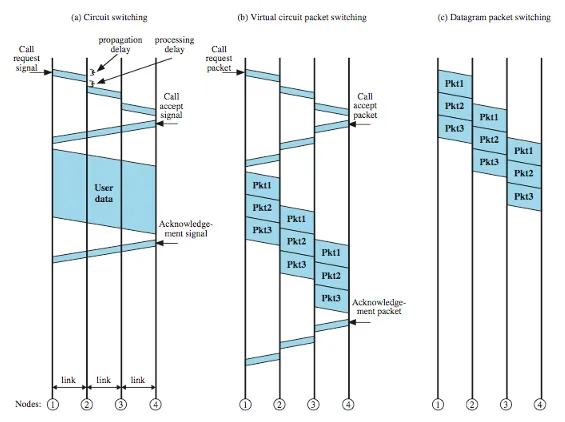
\includegraphics[width=0.8\textwidth]{../assets/ch03/ch03-3_2_交换-002.png}
\end{figure}
图6.2(b)展示了三flit数据包的简单流水线图，假设每个步骤占用一个时钟周期。
将基准微架构扩展至高基数
随着基数增加，集中式分配方法因布线、芯片面积和延迟的急剧增加而变得不可行。本节介绍适用于高
端口数量的分布式交换机和虚拟通道分配结构。
通过采用图3所示的分布式可分离分配器设计，我们解决了交换机分配器的可扩展性问题。分配分为三个
阶段：输入仲裁、本地输出仲裁和全局输出仲裁。第一阶段，每个输入控制器中所有就绪的虚拟通道请
求访问交叉开关。每个输入控制器中获胜的虚拟通道通过驱动请求输出端口的二进制代码到一组水平请
求线上，将请求转发至相应的本地输出仲裁器。




Scalable switch allocator architecture. The input arbiters are localized but the output arbiters are
distributed across the router to limit wiring complexity. A detailed view of the output arbiter
corresponding to output k is shown to the right.
在每个输出仲裁器中，输入请求被解码。第二阶段，每个本地输出仲裁器从其管理的m个输入请求（图
6.3中m=8）中选择一个请求（如有）转发至全局输出仲裁器。最后，全局输出仲裁器从k/m个本地输出

                                                                                                       7
仲裁器中选择一个请求（如有）授予其交换机输出访问权。对于极高基数的路由器，两级输出仲裁器可
扩展至更多级。
分布式仲裁器的每个阶段在相对较少的输入（通常不超过16个）上做出仲裁决策，确保每级可在一个时
钟周期内完成。前两级的仲裁是局部的，仅在物理位置相近的请求中选择。最后一级通过全局布线收集
分布式请求信号，使实际仲裁可在本地执行。确定输出的获胜请求者后，授权信号回传至请求的输入虚
拟通道。为确保公平性，每级仲裁器维护一个基于请求轮转的优先级指针。
虚拟通道分配（VA）比交换机分配更复杂，因为待分配的资源数量乘以虚拟通道数v。与通过信用计数跟
踪下游缓冲区可用性的交换机分配不同，虚拟通道分配中下游虚拟通道的可用性未知。理想的虚拟通道
分配器需允许所有输入虚拟通道监控其等待的所有输出虚拟通道状态，但这种分配器的布线复杂度高达
v²k²，成本过高。
基于交换机分配的设计思路，可构建可扩展的虚拟通道分配器架构。输出虚拟通道的状态保存在每个交
叉点，分配也在交叉点进行。但虚拟通道分配涉及推测，即交换机分配在虚拟通道分配完成前启动以减
少延迟。




图4 Block diagram of a (a) baseline crossbar switch and (b) fully buffered crossbar switch.
全缓冲交叉开关
在交换机的交叉点添加缓冲（图4b）可解耦输入和输出的虚拟通道及交换机分配。这种解耦简化了分
配，减少了对推测的需求，并克服了采用分布式推测分配器的基准架构的性能问题。由于输入和输出交
换机分配完全解耦，赢得输入仲裁的flit会立即转发至其输出对应的交叉点缓冲区。在交叉点，执行与无
缓冲交换机相同的本地和全局输出仲裁。但由于flit已在交叉点缓冲，即使输出仲裁失败也无需重新在输
入端仲裁。

                                                                                             8
中间缓冲区与输入虚拟通道关联。交叉点缓冲区实质上是输入缓冲区针对每个输出的扩展，因此无需为
到达交叉点执行虚拟通道分配——flit已持有输入虚拟通道。输出虚拟通道分配分两步进行：首先通过v选
1仲裁器选择每个交叉点的虚拟通道，再通过k选1仲裁器选择与输出通信的交叉点。
为防止交叉点缓冲区溢出，需采用基于信用的流控。每个输入为其行中的每个kv交叉点缓冲区维护独立
空闲计数器。发送flit至缓冲区时，对应计数器递减；计数为零时，禁止发送。当flit离开交叉点缓冲区
时，返回信用以递增输入的空闲计数。交叉点缓冲区的所需大小由信用延迟（从输入计数器递减到信用
返回的空载交换机延迟）决定。
同一输入行的多个交叉点可能在同周期向不同输出发送flit，从而产生多个信用。高效回传这些信用是一
大挑战。为每个交叉点设置专用信用线成本过高，因此同一输入行的所有交叉点共享一条信用返回总
线。返回信用时，交叉点需仲裁总线访问权。信用返回总线仲裁器采用与输出交换机仲裁器相同的本地-
全局分布式仲裁方法。
在交叉点缓冲区充足的情况下，该设计可实现100%容量饱和吞吐量，因为头部阻塞被完全消除。随着交
叉点缓冲量增加，全缓冲架构逐渐接近虚拟输出队列（VOQ）交换机（每个输入为每个输出维护独立缓
冲区）。全缓冲交叉开关相比VOQ的优势在于无需复杂分配器——6.2节讨论的简单分布式分配方案即可
实现100%吞吐量。
然而，全缓冲交换机的高性能以更大的路由器面积为代价。交叉点缓冲量与vk²成正比，随基数增加成为
芯片面积主导因素。存储面积包括交叉点和输入缓冲区，布线面积包括交叉开关本身及仲裁和信用返回
的控制信号面积。基数增加时，交叉开关带宽（及其面积）保持恒定。布线面积随基数增加源于控制复
杂度的提升。基数超过50时，存储面积超过布线面积。

样例：MELLANOX INFINISCALE IV
InfiniBand协会（ITA）长期制定点对点I/O通信规范，逐步发展为高性能网络结构。InfinisScale IV
（IS4）的链路以2.5Gb/s、5Gb/s和10Gb/s的速率异步运行，宽度可为1x或4x，总链路带宽分别为
10Gb/s（SDR）、20Gb/s（DDR）或40Gb/s（QDR）。




                                                               9
图9 IS4交换芯片的框图，该芯片具有36个端口，每个端口支持4至10 Gb/s，总聚合带宽为2.88 Tb/s的
片外带宽。
IS4微架构采用传统的方法，以非阻塞12×12交叉开关为基本构建块。通过3倍复制形成36端口路由器。
InfiniBand结构中每个主机标有本地标识符（LID），每个交叉开关使用48K条目线性转发表（LFT）通过
目标LID索引路由单播数据包。
多个4x端口可聚合为8x或12x端口，提供每方向40、80或120Gb/s带宽。这使得36端口4x QDR路由器可
视为12端口12x QDR（每方向120Gb/s）路由器，为构建胖树或带网络加速的环面网络提供了灵活性。
每个IS4芯片提供16个服务等级（SL），其中SL15保留给称为管理数据报（MAD）的控制消息。SL在包
头中携带且路由过程中不变。每跳执行服务等级到虚拟通道（VL）的分配。IS4支持最多8个独立VL，可
用于路由算法中的死锁避免、性能隔离或服务质量（QoS）。VL采用基于信用的流控管理下游输入缓冲
区空间，绝不会因输入缓冲区拥塞丢弃数据包，而是阻塞发送端。若其他VL在输入缓冲区中有空间，则
可继续流动。除SL15（管理SL）外，网络链路均采用虚拟直通流控（VCT），硬件不提供流控时由软件
实现。




                                                       10
